\documentclass[11pt]{article}
\usepackage[margin=2.5cm]{geometry}
\usepackage[T1]{fontenc}\usepackage[utf8]{inputenc}\usepackage{lmodern}
\usepackage{amsmath}\usepackage{graphicx}\usepackage{booktabs}\usepackage{tikz}
\usetikzlibrary{arrows.meta,positioning,decorations.pathmorphing}
\usepackage[hidelinks]{hyperref}
\hypersetup{pdftitle={A bio-inspired proton-relay mechanism for base-induced polyketide ring closure},pdfauthor={Julian M. Kleber},pdfkeywords={proton relay, Grotthuss mechanism, polyketide cyclisation, aromatase/cyclase, TcmN, WhiE, biomimetic synthesis, tetracycline, continuous flow}}
\title{A Bio-Inspired Proton-Relay Mechanism for Base-Induced Polyketide Ring Closure:\\ a Hypothesis Inspired by the Aromatase/Cyclases TcmN and WhiE\\[6pt]\large Perspective preprint, version 1.0}
\author{Julian M. Kleber\\[2pt]\small sail.black, Berlin, Germany\\\small ORCID: \href{https://orcid.org/0000-0001-5518-0932}{0000-0001-5518-0932}}
\date{27 October 2026}
\begin{document}\maketitle

\begin{abstract}
Aromatic polyketides such as the tetracyclines are built in bacteria by folding a linear poly-$\beta$-carbonyl chain and closing its rings by aldol condensation. Crystal structures of the aromatase/cyclases TcmN and WhiE-ORFVI suggest that a single, protein-held water molecule acts as the base for the first ring closure and returns a proton to the alkoxide afterwards. We propose a bio-inspired extension of this picture for synthesis outside the enzyme. We hypothesise that, in base-induced cyclisation of poly-$\beta$-carbonyl chains in protic media, the proton removed from the active methylene and the proton returned to the alkoxide travel along a chain of hydrogen bonds by successive hops (a Grotthuss-type proton relay). The same relay could pass a proton from one ring closure to the next and so couple the rings into a cascade. We describe the mechanism step by step, set out the evidence that motivates it and the evidence that argues against it, and derive testable predictions: kinetic isotope effects that depend on the number of hops, a dependence on solvent structure at constant base strength, and characteristic deuterium labelling patterns. We also outline a staged computational test. This paper reports no experimental or computational result in support of the mechanism. It states a hypothesis to be tested.
\end{abstract}
\noindent\textbf{Keywords:} proton relay, Grotthuss mechanism, polyketide cyclisation, aldol condensation, aromatase/cyclase, TcmN, WhiE, biomimetic synthesis, tetracycline, continuous flow chemistry

\section{Introduction}
Tetracyclines are broad-spectrum antibiotics. Demand for them varies, and resistance creates a steady need for new derivatives. The convergent route of Myers and co-workers made fully synthetic tetracyclines accessible from a common precursor \cite{charest2005sci,charest2005jacs}. That route needs many steps, protecting groups and cryogenic lithiation, which makes it hard to run as an on-demand continuous process.

Nature takes a shorter path. A type II polyketide synthase assembles a linear poly-$\beta$-carbonyl chain, and aromatase/cyclase enzymes fold it and close the rings by intramolecular aldol condensation \cite{zhou2010}. Without the cyclase the same chain still cyclises, but it gives a mixture of shunt products \cite{shen1996}. Chemists have copied this logic. Harris and Wittek cyclised partially protected poly-$\beta$-ketones under basic conditions to polycyclic aromatics \cite{harris1975}, Krohn and co-workers used the approach for pradimicinone-type quinones \cite{krohn2000}, and Sparr and co-workers have reviewed and extended catalyst-controlled polyketide cyclisations \cite{faseke2020}.

Every aldol ring closure in such a cascade moves protons twice: one proton leaves the active methylene to form the enolate, and one proton arrives at the alkoxide after the new C--C bond has formed. This paper asks how those protons move. We propose that, in protic media, they can travel by a relay of hops through a hydrogen-bonded chain, in the way excess protons move through water \cite{agmon1995,marx1999}. We call this the proton-relay hypothesis.

\section{What the enzymes show}
The aromatase/cyclase TcmN from the tetracenomycin pathway catalyses C9--C14 first-ring and C7--C16 second-ring cyclisation inside a deep pocket \cite{ames2008}. Ames and co-workers proposed Tyr35 and Arg69 as acid and base for the first ring, and Tyr35, Arg82 and an active-site water for the second. Lee, Ames and Tsai revised this mechanism using the related enzyme WhiE-ORFVI \cite{lee2012}. In their proposal a water molecule held by Glu34 and Tyr35 abstracts the C14 proton, Arg69 protonates the C13 enolate oxygen, the enol attacks C9, and the coordinated water then returns a proton to the C9 oxyanion. For the second ring a replenished water molecule plays the base again. ZhuI, an aromatase/cyclase with C7--C12 specificity, shares the pocket-controlled folding \cite{ames2011}.

Not every cyclase works through water. SnoaL, which closes a ring in nogalamycin biosynthesis, uses a single aspartate (Asp121) as a direct acid and base, and the enolate is stabilised by delocalisation over the aromatic system \cite{sultana2004}. Water-mediated proton transfer is therefore one option in nature, not a rule.

\section{The proposed mechanism}
\paragraph{Core hypothesis.} In base-induced ring closure of a poly-$\beta$-carbonyl chain in a protic medium, the proton transfers of the aldol step proceed by a relay of hops along a hydrogen-bonded chain. The chain can be made of solvent molecules (water, alcohols), the conjugate acid of the base, or enol and carbonyl groups of the folded polyketide itself. The enzymatic mechanism above is the limiting case with a chain of one water molecule.

Scheme~\ref{fig:mech} shows the steps for an illustrative model, heptane-2,6-dione, which closes to a six-membered ring. The model was chosen only because its chemistry is textbook. The real targets are longer polyketides (Section~\ref{sec:valid}).
\begin{enumerate}
\item \textbf{Pre-organisation.} Base, hydrogen-bonded chain and the active methylene come together. In a folded polyketide, neighbouring enol and carbonyl groups can form part of the chain.
\item \textbf{Relay deprotonation.} The C--H proton of the active methylene moves to the first chain member, and the excess proton travels along the chain by hops until the base takes it up. The enolate forms.
\item \textbf{Ring closure.} The enolate carbon attacks the carbonyl carbon further down the chain and forms the new C--C bond and an alkoxide.
\item \textbf{Relay reprotonation.} A proton reaches the alkoxide through the same chain, giving the aldol.
\item \textbf{Dehydration and propagation.} Loss of water gives the enone or, in longer chains, the aromatic ring. The proton released in this step can re-enter the chain and serve the next ring closure, so the base acts as a catalyst and successive rings are coupled.
\end{enumerate}
In the classical reference mechanism a discrete base removes the proton directly, and the alkoxide is protonated later by bulk solvent or during work-up, with diffusion between the steps.

\begin{figure}[t]\centering
\begin{tikzpicture}[node distance=0.2cm,>=Stealth]
\node (a) {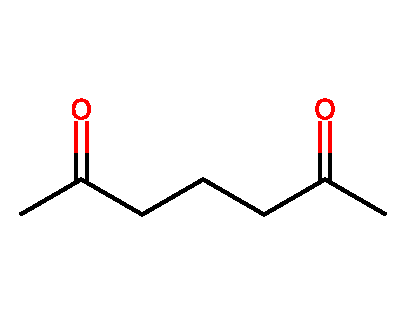
\includegraphics[width=3.2cm]{fig/s1_diketone.pdf}};
\node[right=1.6cm of a] (b) {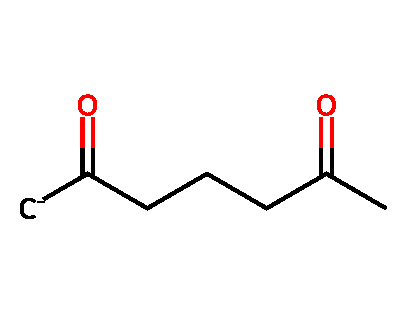
\includegraphics[width=3.2cm]{fig/s2_enolate.pdf}};
\node[right=1.6cm of b] (c) {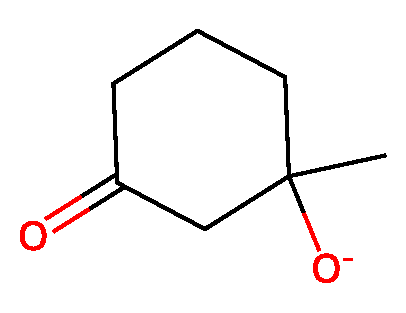
\includegraphics[width=2.6cm]{fig/s3_alkoxide.pdf}};
\node[below=1.4cm of c] (d) {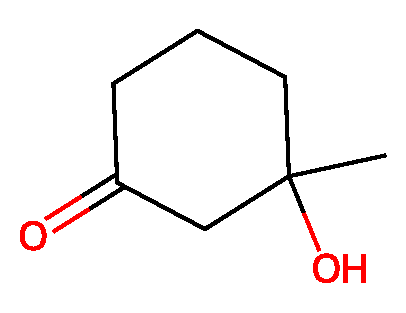
\includegraphics[width=2.6cm]{fig/s4_aldol.pdf}};
\node[left=1.8cm of d] (e) {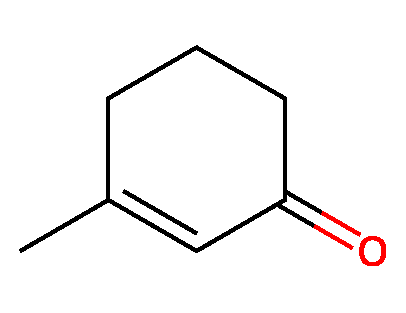
\includegraphics[width=2.6cm]{fig/s5_enone.pdf}};
\draw[->,thick] (a) -- node[above,font=\small,align=center]{(2) relay\\deprotonation} (b);
\draw[->,thick] (b) -- node[above,font=\small,align=center]{(3) ring\\closure} (c);
\draw[->,thick] (c) -- node[right,font=\small,align=left]{(4) relay\\reprotonation} (d);
\draw[->,thick] (d) -- node[above,font=\small,align=center]{(5) $-$H$_2$O} (e);
\end{tikzpicture}
\caption{Proposed steps for an illustrative model, the base-induced intramolecular aldol condensation of heptane-2,6-dione to 3-methylcyclohex-2-en-1-one. Steps (2) and (4) are the proton transfers that the hypothesis assigns to a hydrogen-bond relay (Figure~\ref{fig:relay}). Structures drawn with RDKit.}\label{fig:mech}
\end{figure}

\begin{figure}[t]\centering
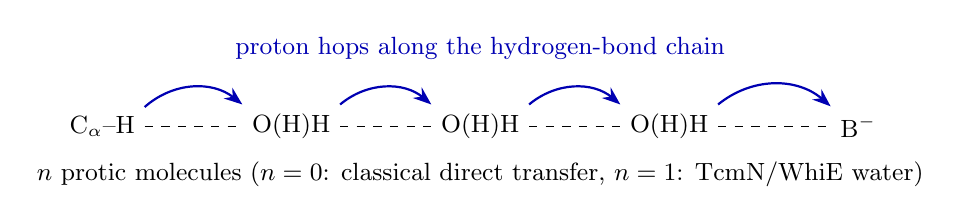
\begin{tikzpicture}[>=Stealth,every node/.style={font=\small}]
\node (c) at (0,0) {C$_\alpha$--H};
\node (w1) at (2.4,0) {O(H)H};
\node (w2) at (4.8,0) {O(H)H};
\node (w3) at (7.2,0) {O(H)H};
\node (b) at (9.6,0) {B$^-$};
\foreach \x/\y in {c/w1,w1/w2,w2/w3,w3/b}{\draw[dashed] (\x) -- (\y);}
\foreach \x/\y in {c/w1,w1/w2,w2/w3,w3/b}{\draw[->,bend left=40,thick,blue!70!black] (\x.north east) to (\y.north west);}
\node[blue!70!black] at (4.8,1.0) {proton hops along the hydrogen-bond chain};
\node at (4.8,-0.6) {$n$ protic molecules ($n=0$: classical direct transfer, $n=1$: TcmN/WhiE water)};
\end{tikzpicture}
\caption{Schematic of relay deprotonation (step 2). Each hop moves a proton to the next acceptor, so the proton that reaches the base is not the one that left C$_\alpha$. Relay reprotonation (step 4) runs the other way, ending at the alkoxide oxygen.}\label{fig:relay}
\end{figure}

\section{Why the hypothesis is plausible}
Proton transport by hopping through hydrogen-bonded networks is established for water \cite{agmon1995,marx1999}. For enolisation in particular, Alagona, Ghio and Nagy computed that one or two water molecules give lower-energy pathways for the keto--enol tautomerism of acetylacetone and pyruvate than direct transfer \cite{alagona2010}. In organocatalysis, a water molecule acting as a proton relay has been examined for the proline-catalysed aldol reaction, and methanol relays have been proposed for related steps \cite{armstrong2014}. The enzymatic mechanism of TcmN and WhiE already places a water molecule between the base and the substrate \cite{ames2008,lee2012}. A folded poly-$\beta$-carbonyl chain carries many enol and carbonyl groups that can donate and accept hydrogen bonds, so the substrate may supply part of its own relay.

\section{What argues against it}
SnoaL closes its ring with direct acid--base catalysis \cite{sultana2004}, so a relay is not required for fast enzymatic aldol cyclisation. Armstrong and co-workers stress that each extra molecule in a transition state costs entropy, and that conclusions based on electronic energies alone can mislead \cite{armstrong2014}. A relay may also be kinetically indistinguishable from general base catalysis in some regimes. Finally, we found no experimental isotope-effect data for base-induced polyketide cyclisations that could already support or exclude the hypothesis.

\section{Relation to prior work}
The enzyme papers \cite{ames2008,lee2012} describe deprotonation, ring closure and reprotonation by a single coordinated water. Computational studies describe water-assisted proton transfer in enolisation and organocatalysis \cite{alagona2010,armstrong2014}. In our literature search (Crossref and web search, October 2026) we did not find a proposal of a multi-hop relay that couples successive ring closures in base-induced polyketide cyclisation, either in enzymes or in synthesis. The new elements here are the multi-hop relay, the coupling of ring closures through the relay, and its use as a design principle for synthesis outside the enzyme. A full database search is still needed before priority can be claimed.

\section{Testable predictions}
\begin{enumerate}
\item[P1] The rate-limiting proton transfer shows a primary H/D kinetic isotope effect. A proton-inventory experiment in H$_2$O/D$_2$O mixtures shows more than one exchangeable proton in flight if a relay operates.
\item[P2] At constant base strength, rate and regioselectivity depend on the hydrogen-bond structure of the solvent, for example the water content of an alcohol or aprotic solvent.
\item[P3] At the same level of theory, computed barriers for relay-assisted deprotonation and reprotonation are lower than those of the direct pathway, after free-energy corrections.
\item[P4] With deuterated active methylenes, deuterium appears at positions of later ring closures if protons are passed from ring to ring.
\end{enumerate}

\section{Proposed computational test}\label{sec:valid}
\begin{enumerate}
\item \textbf{Model relays.} Proton transfer from a $\beta$-diketone active methylene to a base (hydroxide, methoxide, an amine) through chains of 0 to 4 water or methanol molecules, with GFN2-xTB \cite{bannwarth2019} relaxed scans and nudged-elastic-band paths.
\item \textbf{Three substrates.} The platform compound \textbf{10} of the original synthesis plan \cite{kleber2020}, the Krohn polyketide \textbf{12} \cite{krohn2000} (truncated fragments first) and a simple epoxy-polyene as an acid-cascade control \cite{corey1995,hess2017}. Relay and direct paths are compared with density functional theory and implicit plus explicit solvation.
\item \textbf{Dynamics.} Explicit-solvent QM/MM and ab initio molecular dynamics with enhanced sampling along the proton-transfer coordinates.
\item \textbf{Kinetics.} Transition-state-theory rates with tunnelling corrections, H/D isotope effects and proton inventories, to compare with P1 to P4.
\end{enumerate}
The hypothesis is rejected if the relay path is not lower in free energy than the direct path at the same level of theory, or if the difference disappears when functional or solvation model change.

\section{Relevance for continuous flow}
If protons move by relay, the local composition of the protic medium matters as much as the base. A flow reactor controls mixing, residence time, temperature and water content precisely, so it is a natural tool to test P2 and, if the hypothesis holds, to exploit it for selective cascade cyclisations toward tetracycline-type scaffolds \cite{kleber2020}.

\section{Limitations and open questions}
This is a hypothesis paper. It contains no new experimental or computational data, and the scheme uses a textbook model compound for illustration. Several points remain open:
\begin{itemize}
\item The exact structures of platform compound \textbf{10} and of the Krohn polyketide \textbf{12} as simulation inputs still need to be fixed.
\item The base and solvent system for the simulations of \textbf{10} and \textbf{12} is not yet chosen. Conditions of the Harris--Wittek type are one option \cite{harris1975}.
\item The relay may be a single concerted event or a series of hops with shallow intermediates. The computations should decide this.
\item Which molecules form the relay (solvent, conjugate acid of the base or substrate groups) is open.
\item The earlier synthesis plan \cite{kleber2020} cited Nishizawa et al.\ \cite{nishizawa2006} for a cyclisation with a [TiCl$_4$OH]$^-$ counter-ion. The cited paper is titled ``TiCl$_4$ induced anti-Markovnikov rearrangement'', and its relevance to that claim still has to be checked. It is not used as evidence here.
\end{itemize}

\section*{Data and code availability}
The simulation plan and scripts will be released with the first results. This preprint is available under CC BY 4.0 at \url{https://github.com/cap-jmk-launchpad/bioinspired-proton-relay-preprint}.

\section*{Competing interests}
The author declares no competing interests.

\begin{thebibliography}{99}\small
\bibitem{charest2005sci} M.\,G.\ Charest, C.\,D.\ Lerner, J.\,D.\ Brubaker, D.\,R.\ Siegel, A.\,G.\ Myers, A convergent enantioselective route to structurally diverse 6-deoxytetracycline antibiotics, \textit{Science} 2005, 308, 395--398. doi:10.1126/science.1109755
\bibitem{charest2005jacs} M.\,G.\ Charest, D.\,R.\ Siegel, A.\,G.\ Myers, Synthesis of ($-$)-tetracycline, \textit{J.\ Am.\ Chem.\ Soc.} 2005, 127, 8292--8293. doi:10.1021/ja052151d
\bibitem{zhou2010} H.\ Zhou, Y.\ Li, Y.\ Tang, Cyclization of aromatic polyketides from bacteria and fungi, \textit{Nat.\ Prod.\ Rep.} 2010, 27, 839--868. doi:10.1039/b911518h
\bibitem{shen1996} B.\ Shen, C.\,R.\ Hutchinson, Deciphering the mechanism for the assembly of aromatic polyketides by a bacterial polyketide synthase, \textit{Proc.\ Natl.\ Acad.\ Sci.\ USA} 1996, 93, 6600--6604. doi:10.1073/pnas.93.13.6600
\bibitem{harris1975} T.\,M.\ Harris, P.\,J.\ Wittek, Biogenetic-type syntheses of polycyclic polyketide metabolites using partially protected $\beta$-hexa- and $\beta$-heptaketones, \textit{J.\ Am.\ Chem.\ Soc.} 1975, 97, 3270--3271. doi:10.1021/ja00844a085
\bibitem{krohn2000} K.\ Krohn, S.\ Bernhard, U.\ Flörke, N.\ Hayat, Biomimetic-type synthesis of benzo[a]naphthacenequinones related to pradimicinone, \textit{J.\ Org.\ Chem.} 2000, 65, 3218--3222. doi:10.1021/jo9918089
\bibitem{faseke2020} V.\,C.\ Fäseke, F.\,C.\ Raps, C.\ Sparr, Polyketide cyclizations for the synthesis of polyaromatics, \textit{Angew.\ Chem.\ Int.\ Ed.} 2020, 59, 6975--6983. doi:10.1002/anie.201911255
\bibitem{agmon1995} N.\ Agmon, The Grotthuss mechanism, \textit{Chem.\ Phys.\ Lett.} 1995, 244, 456--462. doi:10.1016/0009-2614(95)00905-J
\bibitem{marx1999} D.\ Marx, M.\,E.\ Tuckerman, J.\ Hutter, M.\ Parrinello, The nature of the hydrated excess proton in water, \textit{Nature} 1999, 397, 601--604. doi:10.1038/17579
\bibitem{ames2008} B.\,D.\ Ames, T.\,P.\ Korman, W.\ Zhang, P.\ Smith, T.\ Vu, Y.\ Tang, S.-C.\ Tsai, Crystal structure and functional analysis of tetracenomycin ARO/CYC: implications for cyclization specificity of aromatic polyketides, \textit{Proc.\ Natl.\ Acad.\ Sci.\ USA} 2008, 105, 5349--5354. doi:10.1073/pnas.0709223105
\bibitem{lee2012} M.-Y.\ Lee, B.\,D.\ Ames, S.-C.\ Tsai, Insight into the molecular basis of aromatic polyketide cyclization: crystal structure and in vitro characterization of WhiE-ORFVI, \textit{Biochemistry} 2012, 51, 3079--3091. doi:10.1021/bi201705q
\bibitem{ames2011} B.\,D.\ Ames, M.-Y.\ Lee, C.\ Moody, W.\ Zhang, Y.\ Tang, S.-C.\ Tsai, Structural and biochemical characterization of ZhuI aromatase/cyclase from the R1128 polyketide pathway, \textit{Biochemistry} 2011, 50, 8392--8406. doi:10.1021/bi200593m
\bibitem{sultana2004} A.\ Sultana, P.\ Kallio, A.\ Jansson, J.-S.\ Wang, J.\ Niemi, P.\ Mäntsälä, G.\ Schneider, Structure of the polyketide cyclase SnoaL reveals a novel mechanism for enzymatic aldol condensation, \textit{EMBO J.} 2004, 23, 1911--1921. doi:10.1038/sj.emboj.7600201
\bibitem{alagona2010} G.\ Alagona, C.\ Ghio, P.\,I.\ Nagy, The catalytic effect of water on the keto--enol tautomerism. Pyruvate and acetylacetone: a computational challenge, \textit{Phys.\ Chem.\ Chem.\ Phys.} 2010, 12, 10173--10188. doi:10.1039/c003999c
\bibitem{armstrong2014} A.\ Armstrong, R.\,A.\ Boto, P.\ Dingwall, J.\ Contreras-García, M.\,J.\ Harvey, N.\,J.\ Mason, H.\,S.\ Rzepa, The Houk--List transition states for organocatalytic mechanisms revisited, \textit{Chem.\ Sci.} 2014, 5, 2057--2071. doi:10.1039/c3sc53416b
\bibitem{bannwarth2019} C.\ Bannwarth, S.\ Ehlert, S.\ Grimme, GFN2-xTB: an accurate and broadly parametrized self-consistent tight-binding quantum chemical method with multipole electrostatics and density-dependent dispersion contributions, \textit{J.\ Chem.\ Theory Comput.} 2019, 15, 1652--1671. doi:10.1021/acs.jctc.8b01176
\bibitem{corey1995} E.\,J.\ Corey, S.\,C.\ Virgil, H.\ Cheng, C.\,H.\ Baker, S.\,P.\,T.\ Matsuda, V.\ Singh, S.\ Sarshar, New insights regarding the cyclization pathway for sterol biosynthesis from (S)-2,3-oxidosqualene, \textit{J.\ Am.\ Chem.\ Soc.} 1995, 117, 11819--11820. doi:10.1021/ja00152a030
\bibitem{hess2017} B.\,A.\ Hess, Computational studies on the cyclization of squalene to the steroids and hopenes, \textit{Org.\ Biomol.\ Chem.} 2017, 15, 2133--2145. doi:10.1039/c7ob00222j
\bibitem{nishizawa2006} M.\ Nishizawa, Y.\ Asai, H.\ Imagawa, TiCl$_4$ induced anti-Markovnikov rearrangement, \textit{Org.\ Lett.} 2006, 8, 5793--5796. doi:10.1021/ol062337x
\bibitem{kleber2020} J.\,M.\ Kleber, F5-2 API Synthesis Plan, ResearchGate preprint, 2020. doi:10.13140/RG.2.2.23579.28965
\end{thebibliography}
\end{document}
